% Options for packages loaded elsewhere
\PassOptionsToPackage{unicode}{hyperref}
\PassOptionsToPackage{hyphens}{url}
\PassOptionsToPackage{dvipsnames,svgnames,x11names}{xcolor}
%
\documentclass[
]{article}
\usepackage{amsmath,amssymb}
\usepackage{iftex}
\ifPDFTeX
  \usepackage[T1]{fontenc}
  \usepackage[utf8]{inputenc}
  \usepackage{textcomp} % provide euro and other symbols
\else % if luatex or xetex
  \usepackage{unicode-math} % this also loads fontspec
  \defaultfontfeatures{Scale=MatchLowercase}
  \defaultfontfeatures[\rmfamily]{Ligatures=TeX,Scale=1}
\fi
\usepackage{lmodern}
\ifPDFTeX\else
  % xetex/luatex font selection
\fi
% Use upquote if available, for straight quotes in verbatim environments
\IfFileExists{upquote.sty}{\usepackage{upquote}}{}
\IfFileExists{microtype.sty}{% use microtype if available
  \usepackage[]{microtype}
  \UseMicrotypeSet[protrusion]{basicmath} % disable protrusion for tt fonts
}{}
\makeatletter
\@ifundefined{KOMAClassName}{% if non-KOMA class
  \IfFileExists{parskip.sty}{%
    \usepackage{parskip}
  }{% else
    \setlength{\parindent}{0pt}
    \setlength{\parskip}{6pt plus 2pt minus 1pt}}
}{% if KOMA class
  \KOMAoptions{parskip=half}}
\makeatother
\usepackage{xcolor}
\usepackage[margin=1in]{geometry}
\usepackage{graphicx}
\makeatletter
\def\maxwidth{\ifdim\Gin@nat@width>\linewidth\linewidth\else\Gin@nat@width\fi}
\def\maxheight{\ifdim\Gin@nat@height>\textheight\textheight\else\Gin@nat@height\fi}
\makeatother
% Scale images if necessary, so that they will not overflow the page
% margins by default, and it is still possible to overwrite the defaults
% using explicit options in \includegraphics[width, height, ...]{}
\setkeys{Gin}{width=\maxwidth,height=\maxheight,keepaspectratio}
% Set default figure placement to htbp
\makeatletter
\def\fps@figure{htbp}
\makeatother
\setlength{\emergencystretch}{3em} % prevent overfull lines
\providecommand{\tightlist}{%
  \setlength{\itemsep}{0pt}\setlength{\parskip}{0pt}}
\setcounter{secnumdepth}{-\maxdimen} % remove section numbering
\newlength{\cslhangindent}
\setlength{\cslhangindent}{1.5em}
\newlength{\csllabelwidth}
\setlength{\csllabelwidth}{3em}
\newlength{\cslentryspacingunit} % times entry-spacing
\setlength{\cslentryspacingunit}{\parskip}
\newenvironment{CSLReferences}[2] % #1 hanging-ident, #2 entry spacing
 {% don't indent paragraphs
  \setlength{\parindent}{0pt}
  % turn on hanging indent if param 1 is 1
  \ifodd #1
  \let\oldpar\par
  \def\par{\hangindent=\cslhangindent\oldpar}
  \fi
  % set entry spacing
  \setlength{\parskip}{#2\cslentryspacingunit}
 }%
 {}
\usepackage{calc}
\newcommand{\CSLBlock}[1]{#1\hfill\break}
\newcommand{\CSLLeftMargin}[1]{\parbox[t]{\csllabelwidth}{#1}}
\newcommand{\CSLRightInline}[1]{\parbox[t]{\linewidth - \csllabelwidth}{#1}\break}
\newcommand{\CSLIndent}[1]{\hspace{\cslhangindent}#1}
\setcounter{tocdepth}{3}
\tableofcontents
\fontsize{12}{22}
\selectfont
\usepackage{booktabs}
\usepackage{longtable}
\usepackage{array}
\usepackage{multirow}
\usepackage{wrapfig}
\usepackage{float}
\usepackage{colortbl}
\usepackage{pdflscape}
\usepackage{tabu}
\usepackage{threeparttable}
\usepackage{threeparttablex}
\usepackage[normalem]{ulem}
\usepackage{makecell}
\usepackage{xcolor}
\ifLuaTeX
  \usepackage{selnolig}  % disable illegal ligatures
\fi
\IfFileExists{bookmark.sty}{\usepackage{bookmark}}{\usepackage{hyperref}}
\IfFileExists{xurl.sty}{\usepackage{xurl}}{} % add URL line breaks if available
\urlstyle{same}
\hypersetup{
  pdftitle={Searching spatial-temporal changes in intrinsic productivity of Antarctic Krill (Euphausia superba) in a fishery management context},
  pdfauthor={Mardones Mauricio; George Watters; César Cárdenas},
  colorlinks=true,
  linkcolor={blue},
  filecolor={Maroon},
  citecolor={Blue},
  urlcolor={Blue},
  pdfcreator={LaTeX via pandoc}}

\title{Searching spatial-temporal changes in intrinsic productivity of
Antarctic Krill (Euphausia superba) in a fishery management context}
\usepackage{etoolbox}
\makeatletter
\providecommand{\subtitle}[1]{% add subtitle to \maketitle
  \apptocmd{\@title}{\par {\large #1 \par}}{}{}
}
\makeatother
\subtitle{Working Paper to be submitted in a CCAMLR WG 2023}
\author{Mardones Mauricio\footnote{Instituo de Fomento Pesquero,
  \href{mailto:mardones.mauricio@gmail.com}{\nolinkurl{mardones.mauricio@gmail.com}}} \and George
Watters\footnote{Antarctic División NOAA} \and César
Cárdenas\footnote{Instituto Antártico Chileno}}
\date{14 April, 2024}

\begin{document}
\maketitle

\newpage

\hypertarget{abstract}{%
\section{ABSTRACT}\label{abstract}}

One approach for understanding the dynamics of krill populations in the
Antarctic Peninsula is through the analysis of empirical data, such as
size composition obtained from fishery monitoring. By studying this data
over multiple years and considering life history parameters, we can
assess the intrinsic productivity of krill and potential changes over
time and in different areas. To achieve this, we have employed the
Length-Based Spawning Potential Ratio (LBSPR) method. This method allows
us to estimate the reproductive potential of the population based on
current exploitation levels, as well as its comparison to a virgin
condition. By identifying reference points specifically related to
reproductive potential, the LBSPR method provides insights about the
state of the krill population. Recognizing spatial and temporal changes
in the intrinsic productivity of krill, as indicated by their
reproductive potential, is crucial for the understanding of the unique
characteristics of this species. Moreover, these findings have important
implications for management strategies within the context of the
Commission for the Conservation of Antarctic Marine Living Resources
(CCAMLR). By integrating knowledge of krill dynamics and its
reproductive potential, advise can be produced to ensure the sustainable
management of krill populations in subarea 48.1.

\emph{Keywords: Krill populations, dynamic population, size
compositions, Spawning Potential Ratio (SPR), Management, CCAMLR.}

\newpage

\hypertarget{introduction}{%
\section{1. INTRODUCTION}\label{introduction}}

The western Antarctic Peninsula ecosystem is a critical region of the
Southern Ocean for populations of Antarctic krill (\emph{Euphausia
superba}; hereafter krill) serving as a major spawning and recruitment
area and as an overwintering hotspot, especially within Bransfield
Strait. Over the last 40 years, climate driven changes have resulted in
warming waters, declines in seasonal sea ice extent and duration
{[}\protect\hyperlink{ref-Stammerjohn2008a}{1},\protect\hyperlink{ref-Stammerjohn2008}{2}{]},
changing trends phytoplankton productivity
{[}\protect\hyperlink{ref-Saba2014}{3},\protect\hyperlink{ref-Siegel2013}{4}{]}.

Additionally, changes have impacted the population dynamics of krill,
resulting in distribution changes with consequent contraction of the
population in the southwest Atlantic Ocean toward the peninsula
{[}\protect\hyperlink{ref-Atkinson2009}{5}{]}. In addition, changes in
the population structure have also verified in krill in recent years
{[}\protect\hyperlink{ref-Reiss2020}{6}{]}. The mentioned temporal and
spatial changes have implications for the reproductive potential of the
species and this, therefore, for intrinsic productivity.

One way to understand and measure changes in intrinsic productivity is
through assessing the ratio of krill reproductive potential. There are
many length-based assessment methods to understand this changes between
years
{[}\protect\hyperlink{ref-Rudd2017a}{7}--\protect\hyperlink{ref-Canales2021}{10}{]}.
On the other hand, one of the advantages of these methods is to use one
of the most reliable and abundant sources in the sampling of fishing
activities, such as size structures
{[}\protect\hyperlink{ref-Canales2021}{10}{]}.

Spatial and temporal changes in the population structure have been a
relevant issue within CCAMLR (Commission for the Conservation of
Antarctic Marine Living Resources) fisheries management schemes. In this
sense, new more localized or reduced spatial scales have been proposed
to identify changes in these scales. Despite these proposals to identify
krill population dynamics at a finer level, these schemes are not yet
operational for decision making
{[}\protect\hyperlink{ref-Hill2016}{11},\protect\hyperlink{ref-McBride2021}{12}{]}.

We then propose to identify differences in krill reproductive potential
at the finer spatial and temporal scales, propose a specific reference
point considering the spatial scale, and ultimately provide
recommendations for sustainable management of the krill fishery through
intrinsic productivity in Subarea 48.1 on the Antarctic Peninsula in the
Southern Ocean.

\newpage

\hypertarget{methodology}{%
\section{2. METHODOLOGY}\label{methodology}}

\hypertarget{study-area}{%
\subsection{2.1. Study area}\label{study-area}}

The study area includes subarea 48.1, which is one of the sectors where
today the largest amount of krill fishing is concentrated
{[}\protect\hyperlink{ref-McBride2021}{12}--\protect\hyperlink{ref-SantaCruz2022}{14}{]}.
In order to have a finest spatial definition of krill dynamics
population, we will analyze the differences between the management
strata defined in WG-EMM-2021/05
Rev.~({[}\protect\hyperlink{ref-Dornam2021}{15}{]}), namely Brainsfield
Strait, Elephant Island, Extra, Joinville Island and South West
(hereafter BS, EI, Extra, JOIN and SSIW respectively) (Figure
\ref{Figure 1})

\begin{figure}[H]

{\centering 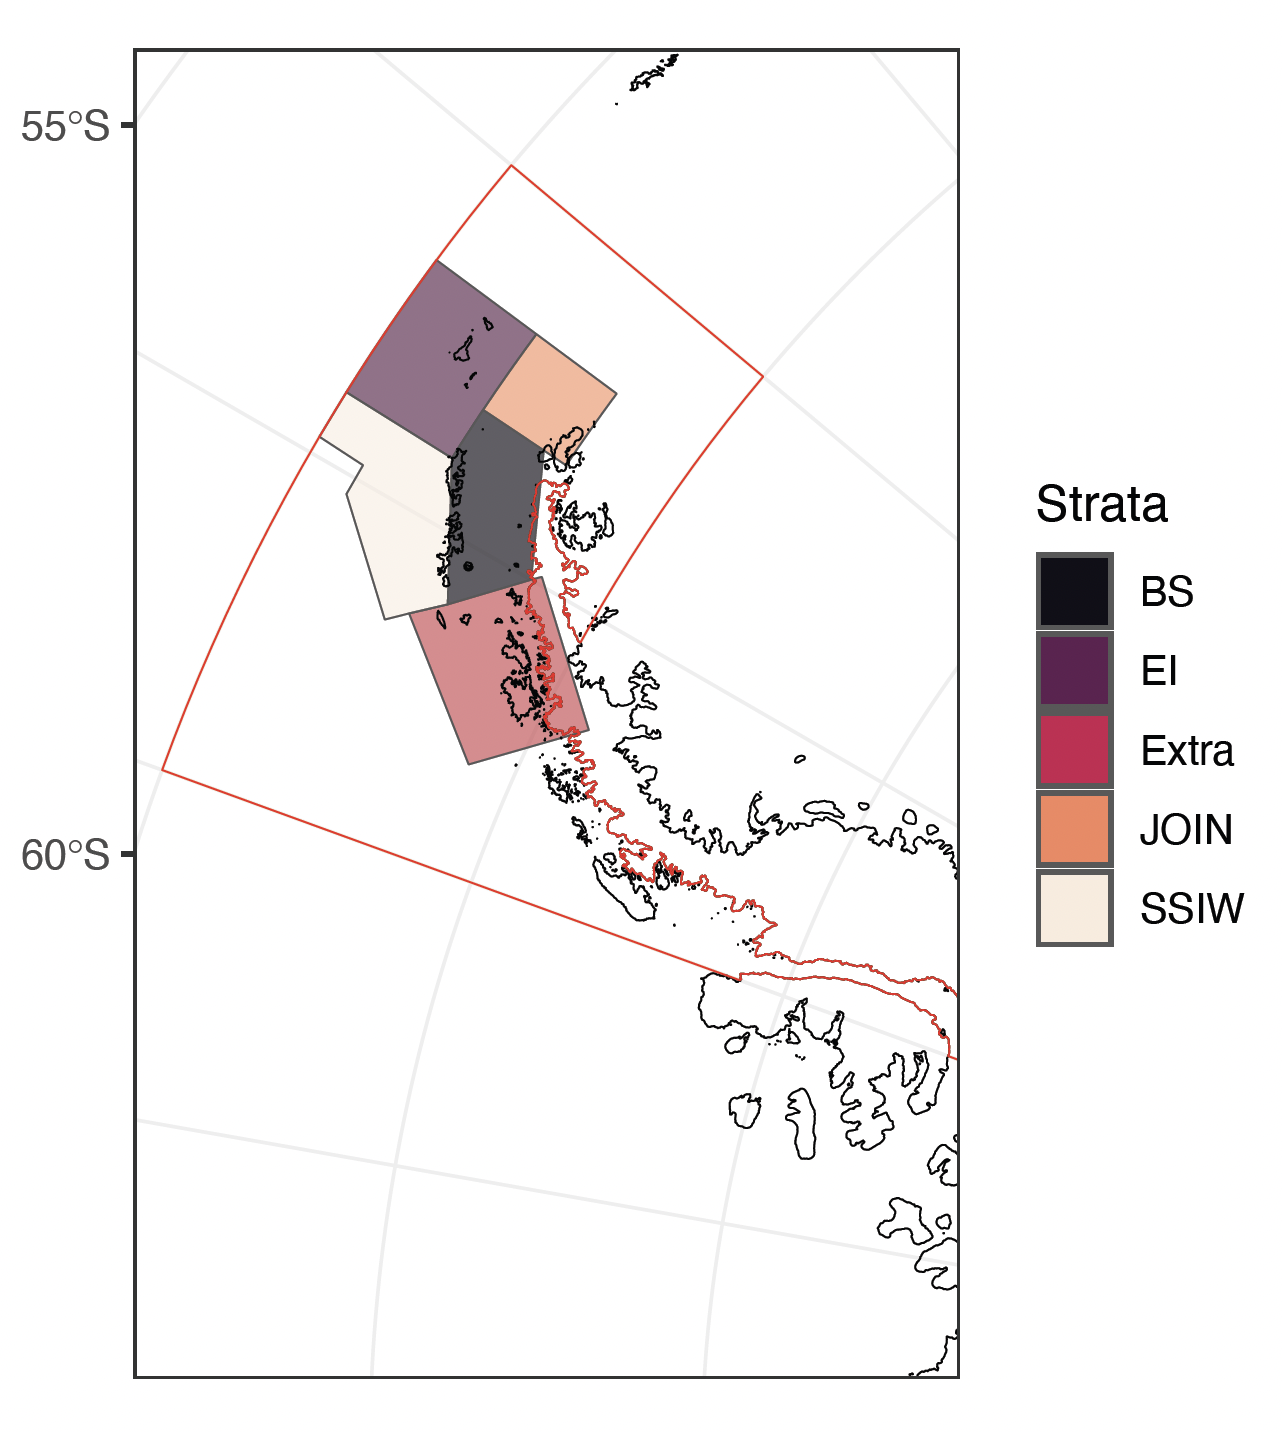
\includegraphics[width=0.6\linewidth]{Strata2} 

}

\caption{\label{Figure 1} Subarea 48.1 and management strata considered in the spatio-temporal analysis of intrinsic productivity of Krill (BS=Brainsfield Strait, EI= Elephant Island, Extra= Extra, JOIN= Joinville Island, SSWI= South West)}\label{fig:Figure 1}
\end{figure}

\hypertarget{monitoring-data-siso-program}{%
\subsection{2.2. Monitoring Data (SISO
Program)}\label{monitoring-data-siso-program}}

For this analysis, data from the monitoring of the krill fishery were
used, which have been systematically collected on board fishing vessels
by the CCAMLR SISO (Scheme of International Scientific Observation)
program. Krill sizes compositions were obtained from the entire area
48.1, which was combined in each management stratum defined at 2.1
section (Figure \ref{Figure 2}).

\begin{figure}[H]

{\centering 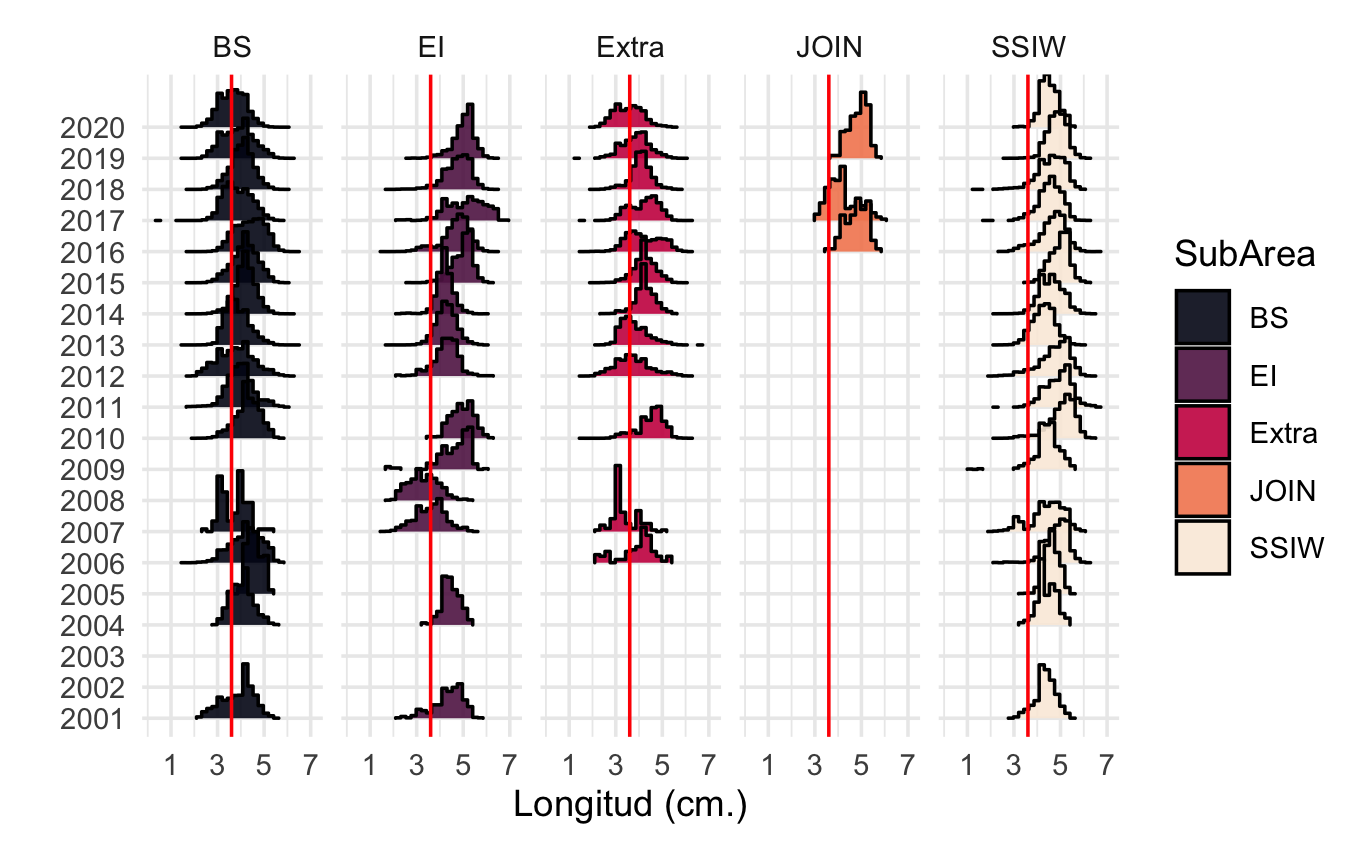
\includegraphics[width=1\linewidth]{tallastrata} 

}

\caption{\label{Figure 2}Sizes compositions from SISO program monitoring krill fishery by strata (BS=Brainsfield Strait, EI= Elephant Island, Extra= Extra, JOIN= Joinville Island, SSWI= South West). Red line represent recruit size}\label{fig:Figure 2}
\end{figure}

The information gaps (years without sizes composition data) are not
calculated because there is no autocorrelation between years, but
singular estimators over time.

\hypertarget{biological-and-fishery-parameters-krill}{%
\subsection{2.3. Biological and fishery parameters
krill}\label{biological-and-fishery-parameters-krill}}

The model needs specifications related to both biological and fishery
parameters according to species evaluated. In a descriptive way, the
main parameter sets are described as follows;

\textbf{Biology}

\begin{itemize}
\tightlist
\item
  von Bertalanffy asymptotic length \texttt{Linf}
\item
  M/K ratio (natural mortality)divided by von Bertalanffy K coefficient)
  \texttt{MK}
\item
  Length at 50\% maturity (\texttt{L50})
\item
  Length at 95\% maturity (\texttt{L95})
\end{itemize}

\textbf{Fishery}

\begin{itemize}
\tightlist
\item
  Length at 50\% selectivity (\texttt{SL50})
\item
  Length at 95\% selectivity (\texttt{SL95})
\item
  Biological Reference Point (BRP). F/M ratio (\texttt{FM}) or Spawning
  Potential Ratio (\texttt{SPR}). If you specify both, the F/M value
  will be ignored.
\end{itemize}

\textbf{Size Classes}

-Width of the length classes (\texttt{BinWidth})

These parameters were taken from previous works about krill life history
and fishery
{[}\protect\hyperlink{ref-Thanassekos2014}{16},\protect\hyperlink{ref-Maschette2020}{17}{]},
which are described (Table \ref{Table1}).

\begin{table}

\caption{\label{tab:table_par}\label{Table1}Krill biological and fishery parameters}
\centering
\begin{tabular}[t]{ll}
\toprule
Value & Descrption\\
\midrule
60 & VB asymptotic length\\
34 & Maturity 50\%\\
55 & Maturity 95\%\\
0.889 & M/K Ratio\\
40 & Selectivity 50\%\\
\addlinespace
56 & Seletivity 95\%\\
0.75 & SPR\\
1 & a (Length-Weight Relation)\\
3.0637 & b (Length-Weight Relation)\\
70 & Bin Min\\
\addlinespace
0 & Bin Max\\
mm & Units\\
\bottomrule
\end{tabular}
\end{table}

\hypertarget{assessment-of-intrinsic-productivity}{%
\subsection{2.4. Assessment of intrinsic
productivity}\label{assessment-of-intrinsic-productivity}}

The intrinsic productivity of krill was evaluated through a method that
measures the reproductive potential of commercially exploited marine
species known as LBSPR (Length Based Spawining Potential Ratio) and
described by {[}\protect\hyperlink{ref-Hordyk2016}{9}{]}. The LBSPR
method has been developed for data-limited fisheries, where few data are
available other than a representative sample of the size structure of
the vulnerable portion of the population (i.e., the catch) and an
understanding of the life history of the species. The Length-Based
Spawning Potential Ratio (LBSPR) method assumes the reproductive
characteristics of the species based on the life history parameters,
being able to establish management strategies for long-lived species
with low reproductive output as well as highly reproductive species with
a high growth constant such as krill
{[}\protect\hyperlink{ref-Prince2018}{18}{]}.

LBSPR uses length-composition data and assumptions about biological
parameters to make a rapid assessment of stock status relative to
unfished levels assuming equilibrium conditions. While LBSPR can use
multiple years of length data, status determination is based on one year
of data at a time (i.e., estimates of status over multiple years are
based on that year's length composition alone). Mean-length mortality
estimators, first developed by
{[}\protect\hyperlink{ref-Beverton1957}{19}{]}, assume that fishing
mortality directly influences mean length of the catch and therefore in
the reproductive potential of the species. Al l this concept about life
history and implications in spawning potential ratio was revisited by
{[}\protect\hyperlink{ref-Jensen1996}{20}{]}.

\hypertarget{model-estimation-lbspr}{%
\subsection{2.5. Model Estimation LBSPR}\label{model-estimation-lbspr}}

Recent work has shown that under equilibrium conditions (that is,
constant F and no recruitment variability) and assuming the von
Bertalanffy growth equation, constant natural mortality for all ages,
and logistic or jack-knife selectivity, standardization of the
composition of lengths of two populations with the same ratio of natural
mortality to growth rate (\emph{M/k}) and the same ratio of mortality by
fishing to natural mortality (\emph{F/M}) will be identical
{[}\protect\hyperlink{ref-Hordyk2016}{9}{]}. Extension of this model to
incorporate length-at-age variability and logistic selectivity confirms
that, at equilibrium, the composition of the predicted duration of catch
of an exploited population is primarily determined by the ratios of M/k
and F/M. The analytical models developed in
{[}\protect\hyperlink{ref-Hordyk2014c}{21}{]} suggest that with
knowledge of the asymptotic von Bertalanffy length \(L_{\infty}\) and
the coefficient of variation in \(CVL_{\infty}\), the ratio of total
mortality to the von Bertalanffy growth coefficient (\emph{Z/k}) for a
given population can be estimated from a representative sample of the
size structure of the catch. If \emph{M/k} (or parameters) is also
known, then the results of {[}\protect\hyperlink{ref-Hordyk2016}{9}{]}
suggest that it is possible to estimate F/M from the composition of the
catch. Often the F/M ratio has been used as a biological reference point
when is 1 {[}\protect\hyperlink{ref-Zhou2012}{22}{]}.

The LBSPR model requires the following parameters: an estimate of the
M/k ratio, \(L_{\infty}\), \(CVL_{\infty}\), and knowledge of maturity
by length (maturity ogive), both set parameters know in krill. This
model uses data on composition by catch sizes to estimate intrinsic
productivity or Spawning Potential Ratio (SPR). This concept was
extracted from {[}\protect\hyperlink{ref-Goodyear1993}{23}{]}, where the
ratio of lifetime average egg production per recruit (EPR) was
calculated for fish and non-fish resources. An algorithm route for the
calculation of the SPR is the following;

\[{SPR}=\frac{EPR_{fished}}{EPR_{nofished}}\] where;

\[
EPR_{fished} =
\sum_{a}
\begin{cases}
 E_{a},  a = 0  \\
 e^{-Z_{{a-1}}a} {E_a}, 0 < a  < a_\le{max}
 \end{cases}       
\] where \(Z_a\) = \(M+F_a\), and \(E\) is egg production at age assumed
to be proportional to weight;

\[E_a \in  Mat_a W_a\] on the other hand, the calculation of the
reproductive potential is the same as that of those captured without F;
\[
EPR_{nofished} =
\sum_{a}
 E_ae^{-M_a}
\] Assuming that egg production is proportional to the size of mature
fish, relative fecundity-at-size is given by;

\[
Fec_{L,g} = Mat_{L,g} L^b
\] where b is value of the exponent to reflect differente size
fecunditity relationship and g is the fraction of recruits to group.

Assuming reasonable estimates of the M/K ratio, \(L_{\infty}\) (or
\(CVL_{\infty}\)), size-at-maturity, the parameters F/M, \(SL_{50}\),
and \(SL_{95}\) can be estimated from a representative sample of the
length structure of the catch by minimizing the following multinomial
negative loglikelihood function (NLL):

\[
NLL =
argmin\sum_{i}
 O_i ln\frac{\hat{P}_i}{\hat{O}_i}
\]

where \(O_i\) and \(\hat{O}_i\) are the observed number and proportion
in length class i, respectively, and \(\hat{P}_i\) is the model estimate
of the probability in length class i
{[}\protect\hyperlink{ref-Hordyk2016}{9}{]}.

Like any assessment method, the LBSPR model relies on a number of
simplifying assumptions. In particular, the LBSPR models are both
equilibrium based and that the length composition data is representative
of the exploited population at steady state
{[}\protect\hyperlink{ref-Hordyk2016}{9},\protect\hyperlink{ref-Hordyk2014c}{21}{]}.
This methodology was implemented through the package
{[}\protect\hyperlink{ref-Hordyk2014c}{21},\protect\hyperlink{ref-LBSPR2021}{\textbf{LBSPR2021?}}{]}
and this code and data could be visited in
\href{https://github.com/MauroMardones/LBSPR_Krill}{LBSPRKrill}.

\hypertarget{biological-references-point-pbr-in-krill.}{%
\subsection{2.6. Biological References Point (PBR) in
krill.}\label{biological-references-point-pbr-in-krill.}}

A constant challenge for krill has been to provide indicators of stock
status that can be compared to predetermined biological reference
points. The intrinsic productivity or SPR is commonly used to set the
limit and target reference point
{[}\protect\hyperlink{ref-Goodyear1993}{23}--\protect\hyperlink{ref-Prince2014}{25}{]}.
By definition, the SPR is equal to 100\% in an unexploited stock, and
zero in a non-spawning stock (eg all mature fish have been removed, or
all females have been caught). The F40\%, that is, the fishing mortality
that allows an escape of 40\% of the biomass to MSY, is the fishing
mortality rate that translates into SPR = 40\%, is considered a
reference point to many species
{[}\protect\hyperlink{ref-Clark2002}{26}{]}. Suitable SPR biological
points can be derived from hypotheses about the steepness of the
stock-recruit relationship
{[}\protect\hyperlink{ref-Hordyk2016}{9},\protect\hyperlink{ref-Brooks2013}{27}{]}.

However {[}\protect\hyperlink{ref-Prince2014}{25}{]} provide some
considerations in relation to the life strategy of the organisms and the
SPR necessary to ensure the sustainability of the fishery. In this work,
three types (I, II and III) are identified, which refers to the r and K
life strategy. The krill is Type 1 (r-strategy), M/k=\textasciitilde1
(m=0.4, k =0.43) therefore, it requires a higher save of SPR.

On the other hand, the current krill fisheries management schemes
established by {[}\protect\hyperlink{ref-CCAMLR2010}{28}{]},
{[}\protect\hyperlink{ref-Constable2000}{29}{]} proposes a decision rule
scheme based on biomass that ensure the sustainability of this resource
in the Southern Ocean. Through a simulation process, a 20-year
projection of the krill population is generated, and a probability
distribution is established around two decision rules. The first rule is
based on the lowest level of exploitation allowed, around 20\% of
biomass, which could be consider a limit reference point. The second is
the target level of the fishery, which indicates the statistical
distribution of the biomass at the end of the 20-year projection under a
constant catch that allows the average escape of 75\% at pre-exploited
levels (CCAMLR-2000 Survey). Linking this management scheme to intrinsic
productivity of krill, we used two reference points for intrinsic krill
productivity, 20\% SPR as the limit reference point and 75\% as the
target to this fishery.

With this references points we can test a challenge for fishing
exploitation and sustainability of krill in the Antarctic Peninsula,
which is related to overfishing by recruitment. This condition occurs
when the adult (reproductive) fraction has been severely reduced due to
excessive fishing, jeopardizing the success of recruitment and stock
replenishment in order to ensure sustainability
{[}\protect\hyperlink{ref-Cubillos2005}{30},\protect\hyperlink{ref-HilbornWalters92}{31}{]}
in relation to the previously mentioned PBRs.

The LBSPR package can be used to generate the expected size composition,
the SPR, and relative yield for a given set of biological and
exploitation pattern parameters. The output of the \texttt{LBSPRsim}
function is an object of class \texttt{LB\_obj}. This is another LBSPR
object, and contains all of the information from the \texttt{LB\_pars}
object and the output of the \texttt{LBSPRsim} function.

It is important to note that the F/M ratio reported in the LBSPR model
refers to the apical F over the adult natural mortality rate. That is,
the value for fishing mortality refers to the highest level of F
experienced by any single size class
{[}\protect\hyperlink{ref-Hordyk2014c}{21}{]}. If the selectivity
pattern excludes all but the largest individuals from being exploited,
it is possible to have a very high F/M ratio in a sustainable fishery
(high SPR) and visceverse. Note that only the life history parameters
need to be specified for the estimation model. The exploitation
parameters will be estimated
{[}\protect\hyperlink{ref-Hordyk2014c}{21}{]}.

Two objects are required to fit the LBSPR model to length data:
life-history parameters (\texttt{LB\_pars}) described previously (2.4.
section) and size compositions (\texttt{LB\_lengths}), which contains
the length frequency data. We provide a set of global size data and also
by strata, with which we will be able to identify the spatial
differences of the potential.

However, it is probably easier to create the \texttt{LB\_lengths} object
by directly reading in a \texttt{.csv}. A length frequency data of krill
set with multiple years (2001-2020) by strata in 48.1 Subarea.

\hypertarget{sensitivity-and-perfomance-analysis.}{%
\subsection{2.7. Sensitivity and perfomance
analysis.}\label{sensitivity-and-perfomance-analysis.}}

Ten sensitivity scenarios based on the upper and lower range for the
asymptotic length von Bertalanffy \(L_{\infty}\) (55 to 65 mm) used in
the base model (60 mm) were tested to identify the impact of this
parameter on the SPR estimation, given that it is the parameters
exhibiting the high degree of variability and one of the factors that
most determines the estimates. On the other hand, the interdependence
between krill and their environment is a well-known and influential
factor in population dynamics, ecosystem impacts, and fishery. This
interdependence also affects the reproductive potential and
consequently, to any management decision that takes into account
population parameters of krill. To assess the impact of individual
growth variability, three scenarios of the VB k parameter were tested,
representing different growth types (low = 0.2, medium = 0.7, and high =
1.2). Figure \ref{Figure3} displays a theoretical growth curve for krill
based on three scenarios that were tested using LBSPR.

\begin{figure}[H]

{\centering \includegraphics{indexPDF_files/figure-latex/Figure 3-1} 

}

\caption{\label{Figure3}Theoretical growth scenarios to krill varability}\label{fig:Figure 3}
\end{figure}

After applying each scenario using each of the parameter setting, the
results of scenarios are compared with the results provided by the
methods based setting (Table 1), analyzing in this way the efect of
underestimation/overestimation of the parameters \(L_{\infty}\) and
\emph{k}.

\newpage

\hypertarget{results}{%
\section{3. RESULTS}\label{results}}

\hypertarget{model-perfomance}{%
\subsection{3.1. Model Perfomance}\label{model-perfomance}}

The results demonstrate good fits of the size structure distribution
model for krill across the strata. The model accurately captures the
distribution patterns of size classes, indicating its effectiveness in
characterizing the population structure. The model successfully captures
the variations in size distribution, reflecting the natural variability
in krill populations across different strata. These findings suggest
that the model can be utilized as a valuable tool for understanding and
predicting size structure dynamics in krill populations (Figure
\ref{Figure4}).

\begin{figure}[H]

{\centering \includegraphics{indexPDF_files/figure-latex/unnamed-chunk-9-1} 

}

\caption{\label{Figure4}Fit of the model to the data of lengths in Braishfield strata}\label{fig:unnamed-chunk-9}
\end{figure}

The Joinville strata exhibits the least model fits, supposedly
attributed to the limited available size compositions data spanning only
three years (Figure \ref{Figure5}).

\begin{figure}[H]

{\centering 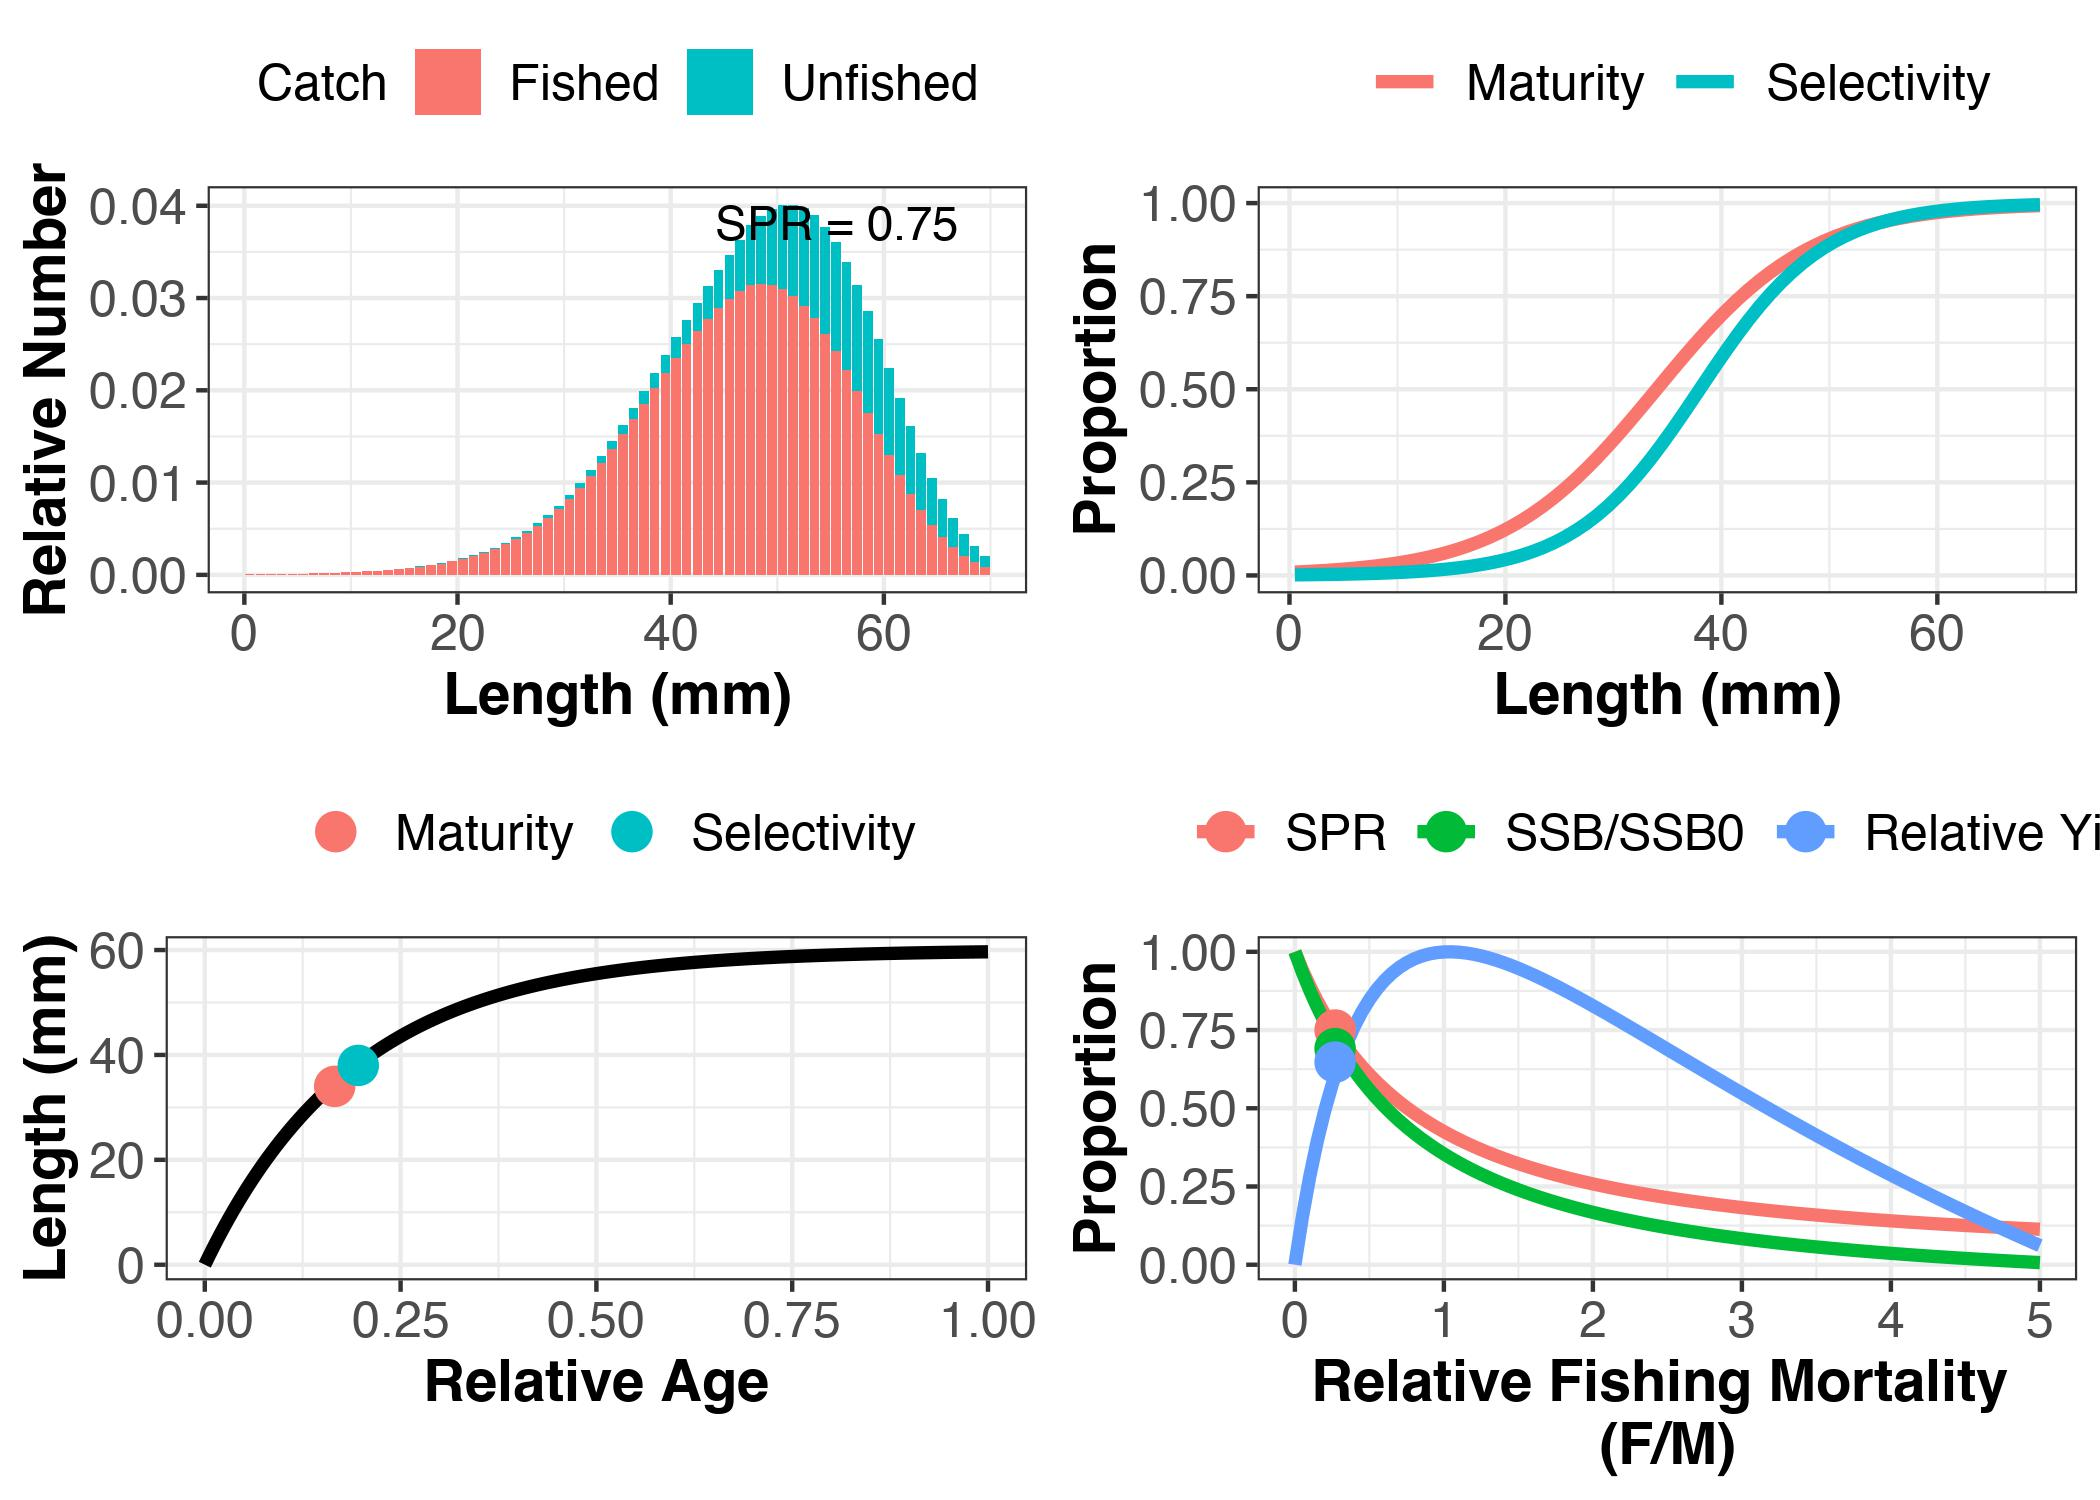
\includegraphics{indexPDF_files/figure-latex/unnamed-chunk-10-1} 

}

\caption{\label{Figure5}Fit of the model to the data of lengths in Joinville strata}\label{fig:unnamed-chunk-10}
\end{figure}

For all the other strata (Extra, EI and SSWI) the model predict sizes
compositions in a correct way for all the years (for details see
\href{https://github.com/MauroMardones/LBSPR_Krill}{LBSPRKrill}).

The difference between the observed accumulated size compositions for
each stratum and compare it with the expected size composition at a
target SPR (75\% SPR). In the simulation of the structure in its virgin
condition (without fishing), the red bars represent each stratum.
Additionally, the overlap with the average structures observed during
the years of fishery monitoring can be visualized. The SSWI Extra and EI
strata exhibit the greatest differences from the simulated structure,
possibly due to the significant contribution of juveniles in these
strata. Conversely, the BS and JO strata demonstrate the closest
resemblance to the simulated structure (Figure \ref{Figure6}).

\begin{figure}[H]

{\centering 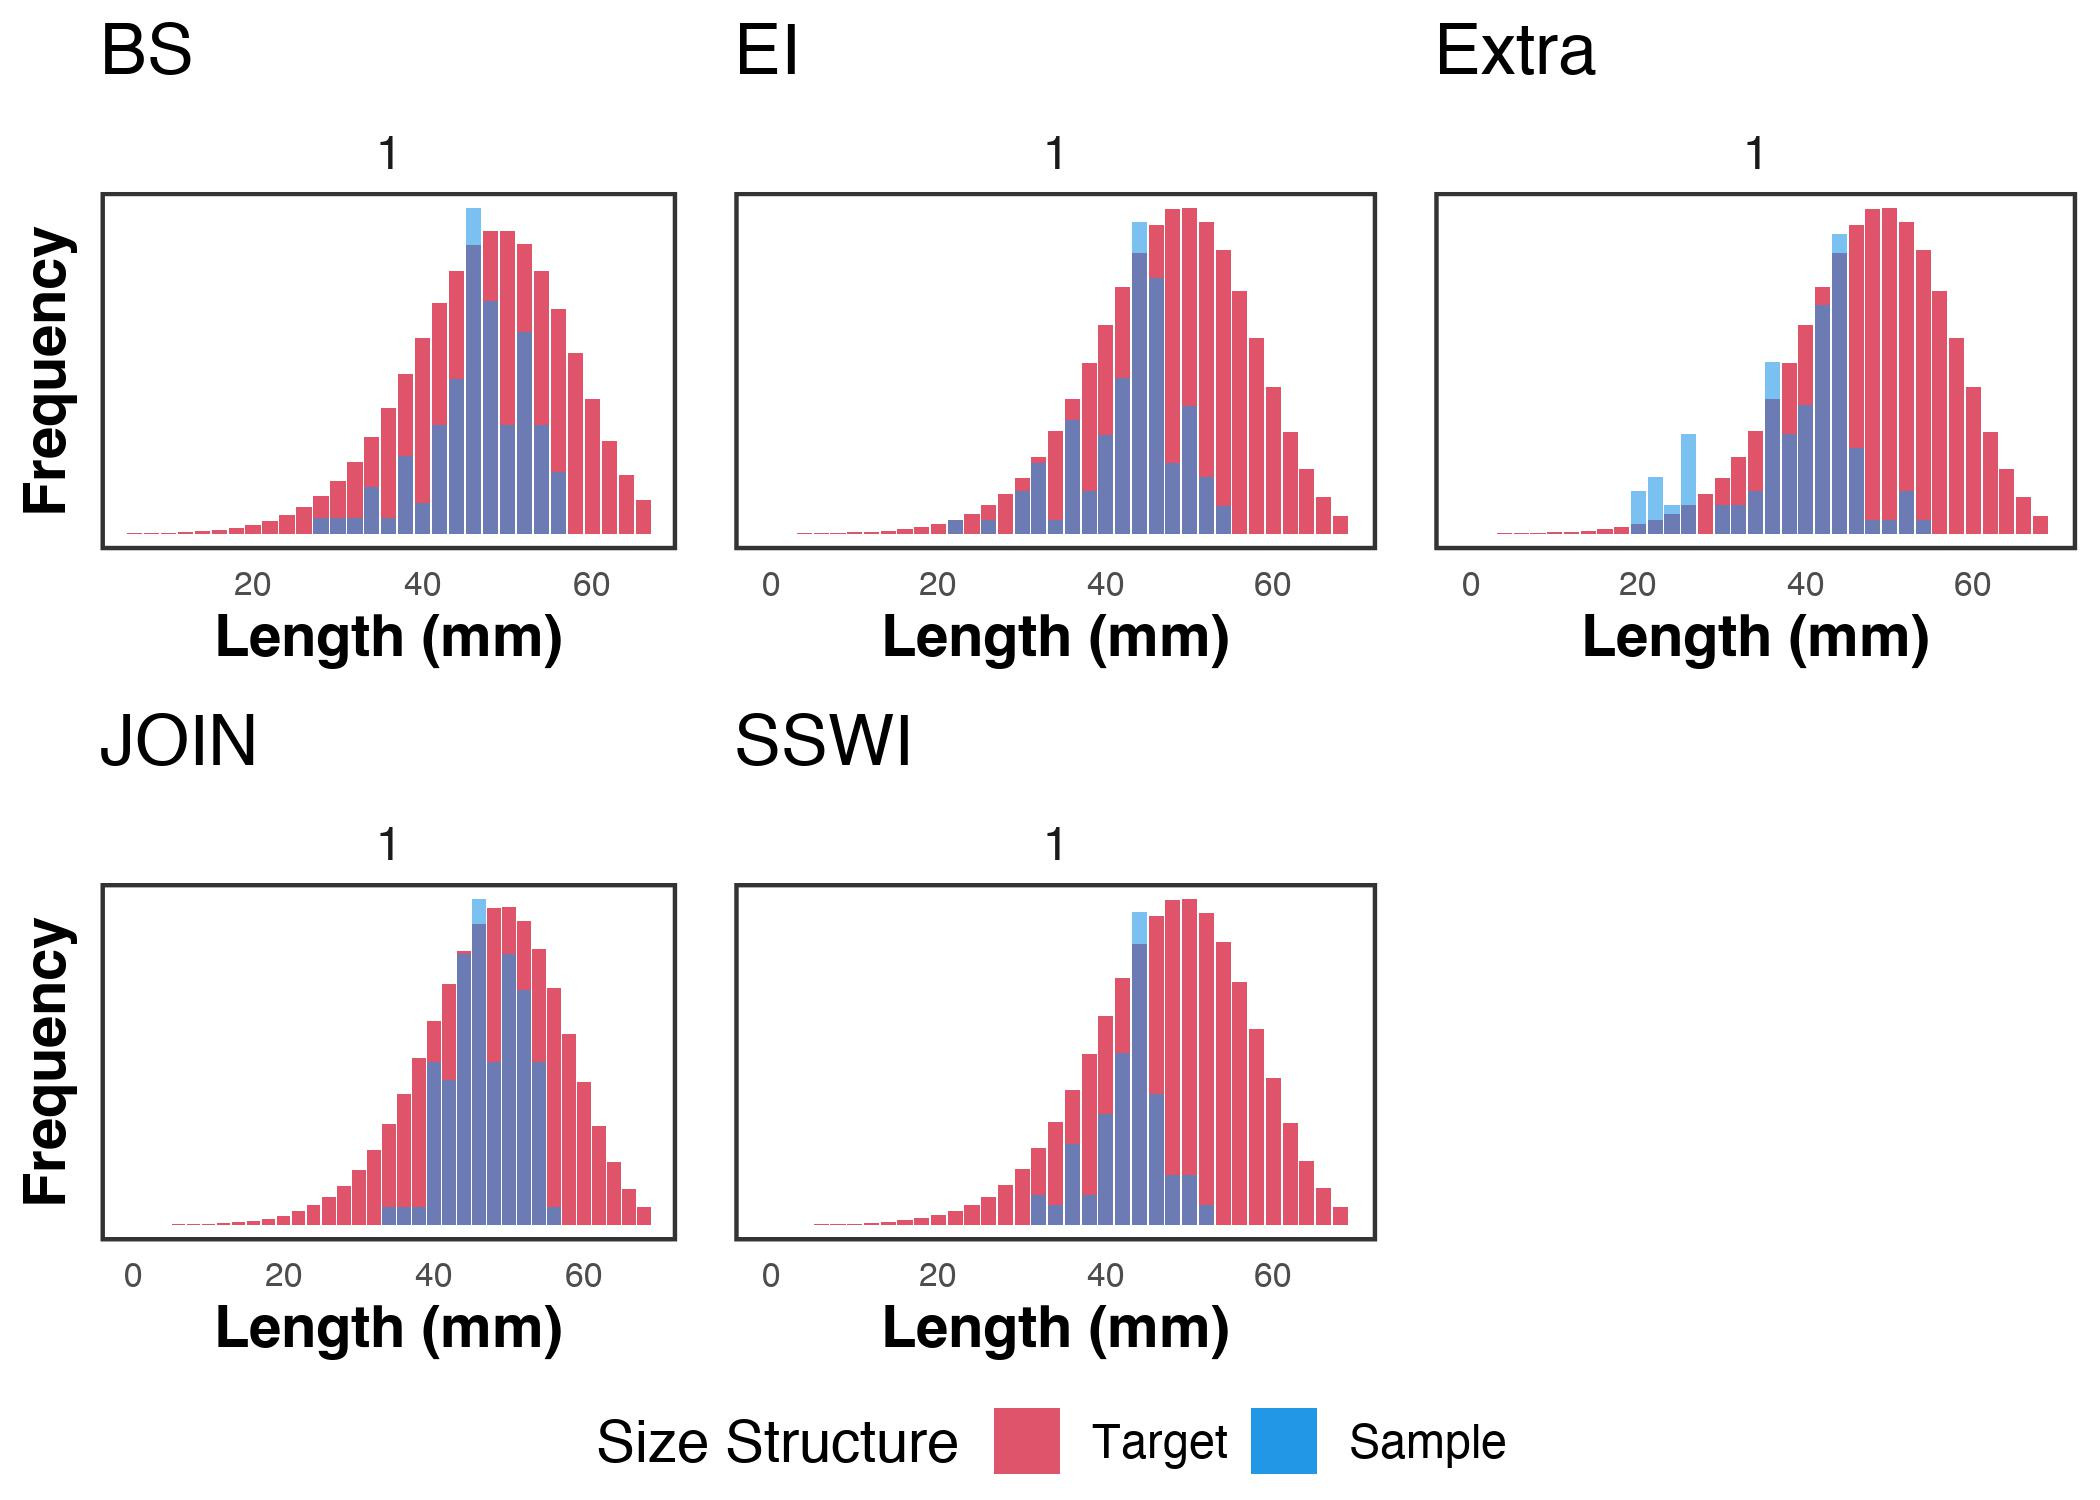
\includegraphics{indexPDF_files/figure-latex/unnamed-chunk-12-1} 

}

\caption{\label{Figure6}Difference between the observed accumulated size structure for each stratum related SPR objective}\label{fig:unnamed-chunk-12}
\end{figure}

Furthermore, ogive maturity curve specific to each stratum and year, as
well as the estimated length selectivity curve, are presented in Figure
\ref{Figure7}. These curves offer crucial insights into the fishery's
impact on the population and its reproductive status, providing measures
of the population's vulnerability to fishing mortality. Notably, the
Braisnfield stratum stands out with a lower proportion of mature
individuals, suggesting a higher prevalence of juveniles. It is
important to note that the same maturity parameters were applied across
all strata.

\begin{figure}[H]

{\centering \includegraphics{indexPDF_files/figure-latex/curve_mat-1} 

}

\caption{\label{Figure7}Maturity curves by strata}\label{fig:curve_mat}
\end{figure}

\hypertarget{comparing-producivity-between-years-and-stratas}{%
\subsection{3.2. Comparing producivity between years and
Stratas}\label{comparing-producivity-between-years-and-stratas}}

The analysis of the krill population's reproductive potential across
different years and strata reveals significant differences. Brainsfield
and Extra strata exhibit a low reproductive potential below the proposed
management target of 75\% in the last year, with values of 0.121 and
0.085, respectively, falling even below the limit reference point. This
condition arises from the concentration of a substantial number of
immature individuals (juveniles) in these strata, which are being
exploited by the fishery, thereby hindering their reproductive cycles
from completing. On the contrary, the Elephant Island stratum
demonstrates higher spawning potential ratio (SPR) levels in recent
years, reaching 0.421 in 2019, which aligns closer to the management
objective. This discrepancy is attributed to the spatial distribution of
krill, as the Elephant Island stratum possesses a larger proportion of
adult individuals compared to other strata. Figure \ref{Figure8}
provides a visual representation of the SPR trends across years and
strata, clearly indicating the references (yellow line = 75\% SPR
Objective and Red line = 20\% Limit SPR).

\begin{figure}[H]

{\centering \includegraphics{indexPDF_files/figure-latex/unnamed-chunk-15-1} 

}

\caption{\label{Figure8}Krill Intrinsic Productivity (SPR) by strata and by year}\label{fig:unnamed-chunk-15}
\end{figure}

The Elephant Island stratum has exhibited a higher prevalence of adult
fraction in fishing catches, leading to an increase in reproductive
potential in recent years. Conversely, the Bransfield and Extra strata
experience intense recruitment overfishing, with their reproductive
potential falling significantly below the recommended target at 54\% and
66.5\%, respectively.

All the estimated values of SPR and their associated variance by stratum
and by year can be identified in Table \ref{Table2}.

\begin{table}

\caption{\label{tab:unnamed-chunk-16}\label{Table2}Estimates SPR by Strata}
\centering
\fontsize{10}{12}\selectfont
\begin{tabu} to \linewidth {>{\raggedleft}X>{\raggedleft}X>{\raggedleft}X>{\raggedleft}X>{\raggedleft}X>{\raggedleft}X>{\raggedleft}X>{\raggedleft}X>{\raggedleft}X>{\raggedleft}X>{\raggedleft}X}
\toprule
\multicolumn{1}{c}{ } & \multicolumn{5}{c}{SPR} & \multicolumn{5}{c}{Variance} \\
\cmidrule(l{3pt}r{3pt}){2-6} \cmidrule(l{3pt}r{3pt}){7-11}
Year & SPR BS & SPR EI & SPR Extra & SPR JOIN & SPR SSWI & Var BS & Var EI & Var Extra & Var JOIN & Var SSWI\\
\midrule
2001 & 0.339 & 0.223 & NA & NA & 0.194 & 0.025 & 0.017 & NA & NA & 0.003\\
2004 & 0.209 & 0.221 & NA & NA & 0.210 & 0.003 & 0.001 & NA & NA & 0.002\\
2005 & 0.325 & NA & NA & NA & 0.254 & 0.001 & NA & NA & NA & 0.000\\
2006 & 0.314 & NA & 0.152 & NA & 0.353 & 0.026 & NA & 0.008 & NA & 0.033\\
2007 & 0.372 & 0.090 & 0.069 & NA & 0.274 & 0.024 & 0.002 & 0.000 & NA & 0.017\\
\addlinespace
2008 & 0.125 & 0.072 & NA & NA & NA & 0.002 & 0.001 & NA & NA & NA\\
2009 & 0.296 & 0.319 & NA & NA & 0.234 & 0.003 & 0.011 & NA & NA & 0.001\\
2010 & 0.310 & 0.424 & 0.246 & NA & 0.457 & 0.006 & 0.027 & 0.019 & NA & 0.013\\
2011 & 0.579 & NA & NA & NA & 0.417 & 0.010 & NA & NA & NA & 0.014\\
2012 & 0.395 & 0.176 & 0.149 & NA & 0.362 & 0.061 & 0.006 & 0.001 & NA & 0.017\\
\addlinespace
2013 & 0.193 & 0.182 & 0.128 & NA & 0.182 & 0.001 & 0.001 & 0.000 & NA & 0.003\\
2014 & 0.235 & 0.157 & 0.177 & NA & 0.294 & 0.001 & 0.000 & 0.001 & NA & 0.002\\
2015 & 0.247 & 0.385 & 0.182 & NA & 0.378 & 0.005 & 0.016 & 0.001 & NA & 0.023\\
2016 & 0.331 & 0.317 & 0.294 & 0.331 & 0.301 & 0.029 & 0.029 & 0.003 & 0.036 & 0.026\\
2017 & 0.211 & 1.000 & 0.190 & 0.254 & 0.262 & 0.008 & 0.000 & 0.015 & 0.002 & 0.007\\
\addlinespace
2018 & 0.216 & 0.330 & 0.132 & NA & 0.291 & 0.002 & 0.034 & 0.001 & NA & 0.033\\
2019 & 0.331 & 0.421 & 0.125 & 0.345 & 0.367 & 0.010 & 0.018 & 0.002 & 0.023 & 0.002\\
2020 & 0.121 & NA & 0.085 & NA & 0.240 & 0.002 & NA & 0.001 & NA & 0.001\\
\bottomrule
\end{tabu}
\end{table}

\newpage

\hypertarget{sensitivity-and-perfomance-analysis}{%
\subsection{3.3. Sensitivity and perfomance
analysis}\label{sensitivity-and-perfomance-analysis}}

The results of the methods in the reference setting are compared to the
obtained under overstimation/underestimation in intrinsic productivity
regarding asymptotic length von Bertalanffy \(L_{\infty}\) parameter in
krill. First, it was possible to identify that for all strata, the
impact of low \(L_{\infty}\) ranges under the base model (60 mm)
overestimates the level of reproductive potential krill with values
between 42\% and 32\% (Bransfield and Elephant Island strata
respectively). Regarding higher \(L_{\infty}\) settings, the model tends
to underestimate the reproductive potential with values between -25\%
and -30\% (Extra and Joinville strata) (Figure \ref{Figure9}, Table
\ref{Table3}).

\begin{figure}[H]

{\centering \includegraphics{indexPDF_files/figure-latex/unnamed-chunk-20-1} 

}

\caption{\label{Figure9}lSensitivity analysis by strata about asymptotic length VB}\label{fig:unnamed-chunk-20}
\end{figure}

\begin{table}

\caption{\label{tab:unnamed-chunk-21}\label{Table3}Estimated by asymptotyc lenght (VB) scenario}
\centering
\fontsize{10}{12}\selectfont
\begin{tabu} to \linewidth {>{\raggedright}X>{\raggedleft}X>{\raggedleft}X>{\raggedleft}X>{\raggedleft}X>{\raggedleft}X>{\raggedleft}X>{\raggedleft}X>{\raggedleft}X>{\raggedleft}X>{\raggedleft}X}
\toprule
\multicolumn{1}{c}{ } & \multicolumn{5}{c}{SPR} & \multicolumn{5}{c}{Variance} \\
\cmidrule(l{3pt}r{3pt}){2-6} \cmidrule(l{3pt}r{3pt}){7-11}
VB scenario & Median BS & Median EI & Median Extra & Median JOIN & Median SSWI & Variance BS & Variance EI & Variance Extra & Variance JOIN & Variance SSWI\\
\midrule
Linf55 & 0.50 & 0.45 & 0.26 & 0.50 & 0.47 & 0.05 & 0.06 & 0.01 & 0 & 0.02\\
Linf56 & 0.43 & 0.41 & 0.23 & 0.45 & 0.43 & 0.04 & 0.06 & 0.01 & 0 & 0.01\\
Linf57 & 0.39 & 0.38 & 0.21 & 0.40 & 0.39 & 0.03 & 0.05 & 0.01 & 0 & 0.01\\
Linf58 & 0.35 & 0.35 & 0.19 & 0.37 & 0.35 & 0.02 & 0.05 & 0.01 & 0 & 0.01\\
Linf59 & 0.31 & 0.33 & 0.18 & 0.34 & 0.32 & 0.01 & 0.05 & 0.00 & 0 & 0.01\\
\addlinespace
Linf60 & 0.29 & 0.31 & 0.16 & 0.31 & 0.30 & 0.01 & 0.05 & 0.00 & 0 & 0.01\\
Linf61 & 0.26 & 0.29 & 0.15 & 0.29 & 0.28 & 0.01 & 0.05 & 0.00 & 0 & 0.01\\
Linf62 & 0.25 & 0.27 & 0.14 & 0.27 & 0.26 & 0.01 & 0.04 & 0.00 & 0 & 0.00\\
Linf63 & 0.23 & 0.25 & 0.13 & 0.25 & 0.24 & 0.01 & 0.03 & 0.00 & 0 & 0.00\\
Linf64 & 0.22 & 0.23 & 0.12 & 0.24 & 0.23 & 0.01 & 0.03 & 0.00 & 0 & 0.00\\
\addlinespace
Linf65 & 0.21 & 0.22 & 0.12 & 0.22 & 0.22 & 0.01 & 0.02 & 0.00 & 0 & 0.00\\
\bottomrule
\end{tabu}
\end{table}

Regarding the three growth levels of the species (high, medium, low)
referred to the parameter \(k\), it was possible to identify that high
and medium growth types result in very low SPR (spawning potential
ratio) estimates compared to slow and medium growth. In fact, with high
individual growth, the model estimates that SPR levels would be very
close to the target management levels (75\% SPR) and far from the limit
reference level of 20\% (Figure \ref{Figure10}, Table \ref{Table4}).

\begin{figure}[H]

{\centering \includegraphics[width=0.7\linewidth]{indexPDF_files/figure-latex/unnamed-chunk-25-1} 

}

\caption{\label{Figure10}Sensitivity analysis by strata about krill growth type}\label{fig:unnamed-chunk-25}
\end{figure}

\begin{table}

\caption{\label{tab:unnamed-chunk-26}\label{Table4}Estimated by growth type scenario}
\centering
\fontsize{10}{12}\selectfont
\begin{tabu} to \linewidth {>{\raggedright}X>{\raggedleft}X>{\raggedleft}X>{\raggedleft}X>{\raggedleft}X>{\raggedleft}X>{\raggedleft}X>{\raggedleft}X>{\raggedleft}X>{\raggedleft}X>{\raggedleft}X}
\toprule
\multicolumn{1}{c}{ } & \multicolumn{5}{c}{SPR} & \multicolumn{5}{c}{Variance} \\
\cmidrule(l{3pt}r{3pt}){2-6} \cmidrule(l{3pt}r{3pt}){7-11}
Growth scenario & Median BS & Median EI & Median Extra & Median JOIN & Median SSWI & Variance BS & Variance EI & Variance Extra & Variance JOIN & Variance SSWI\\
\midrule
Low & 0.64 & 0.60 & 0.47 & 0.71 & 0.64 & 0.02 & 0.04 & 0.03 & 0 & 0.01\\
Med & 0.15 & 0.17 & 0.08 & 0.16 & 0.16 & 0.01 & 0.02 & 0.00 & 0 & 0.00\\
High & 0.09 & 0.10 & 0.04 & 0.09 & 0.09 & 0.00 & 0.01 & 0.00 & 0 & 0.00\\
\bottomrule
\end{tabu}
\end{table}

\newpage

\hypertarget{discusion}{%
\section{4. DISCUSION}\label{discusion}}

\hypertarget{changes-in-krill-population-structure}{%
\subsection{4.1. Changes in krill population
structure}\label{changes-in-krill-population-structure}}

Identifying the population dynamics changes of krill in Subarea 48.1 has
been one of the biggest challenges in recent years as temporal-spatial
patterns of both concentration and productivity of catches has
increased, as well environmental changes are already affecting the
ecosystem
{[}\protect\hyperlink{ref-Hill2016}{11},\protect\hyperlink{ref-McBride2021}{12}{]}.
Krill is a key species in the Antarctic environment and understanding
its population dynamics is a basic element to visualize the impacts on
the functioning of the food web, conservation of the resource and
management of the fishery {[}\protect\hyperlink{ref-Hill2016}{11}{]}.
For these reasons, it is key to assess the reproductive potential of the
species at fine scales of space and time in subarea 48.1, because this
area is where the fishery and resource have been concentrated for the
last 20 years
{[}\protect\hyperlink{ref-Atkinson2022}{13},\protect\hyperlink{ref-SantaCruz2022}{14}{]}
and the needs for advises for a sustainable management are currently
required. In this method we determined the differences between the
simulated krill size structures based on their life history parameters
{[}\protect\hyperlink{ref-Maschette2020}{17}{]} and those resulting from
the fishery, which allows us to know the difference between the virginal
reproductive potential and that currently fishing mortality levels.

Our results identify this changes in spatio-temporal variability of
krill in different fishing management strata and, in turn, it was
possible to propose Biological Reference Points based on the
characteristics of the species, which in turn constitutes a
recommendation for the current exploitation strategy carried out by
CCMLAR. In this sense, we identify the historical fishing periods based
on the reproductive potential and, in turn, an explicit spatial
management is proposed based on these results. In recent years, the
identification of population dynamics changes in krill within Subarea
48.1 has posed significant challenges. Temporal-spatial patterns of
catch concentration and productivity have witnessed a notable increase,
while the ecosystem has already begun experiencing the impacts of
environmental changes
{[}\protect\hyperlink{ref-Hill2016}{11},\protect\hyperlink{ref-McBride2021}{12}{]}.
Krill plays a crucial role in the Antarctic environment, and
understanding its population dynamics is fundamental for comprehending
the effects on the food web, conserving the resource, and managing the
fishery {[}\protect\hyperlink{ref-Hill2016}{11}{]}. Given the
concentration of fishing activity and resource abundance in Subarea 48.1
over the past two decades
{[}\protect\hyperlink{ref-Atkinson2022}{13},\protect\hyperlink{ref-SantaCruz2022}{14}{]},
it is vital to assess the krill intrinsic productivity at fine spatial
and temporal scales. This assessment is currently necessary to provide
guidance for sustainable management practices. Our research has
successfully identified spatio-temporal variability changes in krill
across different fishing management strata. Furthermore, based on the
krill population features, we have proposed a Biological Reference
Points, offering recommendations for the current exploitation strategy
conducted by CCAMLR.

Changes in the dynamics and population structure of krill in the
Antarctic Peninsula are manifested in various ways, such as
distribution, biomass, recruitment, phenology, among others. The main
drivers of these changes are associated with the changing behavior of
the different environmental variables in the krill habitat
{[}\protect\hyperlink{ref-Saba2014}{3},\protect\hyperlink{ref-Flores2012a}{32}--\protect\hyperlink{ref-Walsh2020}{36}{]}.
Faced with this changing scenario, the intrinsic population
productivity, that is, the reproductive potential of the species, has
also undergone changes in the last decades
{[}\protect\hyperlink{ref-McBride2021}{12},\protect\hyperlink{ref-Atkinson2022}{13},\protect\hyperlink{ref-Perry2020}{37}{]},
both on the temporal scale as well as the spatial one. Similarly, the
population structure of krill in the PA has been impacted by this type
of environmental forcing
{[}\protect\hyperlink{ref-Siegel2013}{4},\protect\hyperlink{ref-Reiss2020}{6}{]}.
While we understand that recruitment variability is influenced by
environmental factors, including biomass, it is possible to identify the
risk of fishing activity on the reproductive condition of the krill
population over time and space, in other words, the risk of recruitment
overfishing varies across years and strata in Antarctic Peninsula.

\hypertarget{fishery-data-as-population-indicators}{%
\subsection{4.2. Fishery data as population
indicators}\label{fishery-data-as-population-indicators}}

Krill in the PA have been harvested commercially since about 1970 and
constitute the largest fishery in the Southern Ocean. The data on the
fishing activity around krill have been systematically collected on
board the fishing vessels through the SISO program, with which it has
also been possible to identify changes in the population dynamics that
have occurred during the last two decades and throughout the area of
greater exploitation. The accurate representation of size distribution
is crucial for assessing the overall health and productivity of krill
populations and for informing effective management strategies in
different geographical areas
{[}\protect\hyperlink{ref-Thanassekos2014}{16}{]}. Changes in the
availability, distribution, and concentration, performance of the
resource have been reflected in this kind of data
{[}\protect\hyperlink{ref-Froese2018}{8}--\protect\hyperlink{ref-Canales2021}{10}{]}.
To identify changes in the intrinsic productivity of the krill
population, we used one of the most representative pieces of information
on the population dynamics of exploited marine resources that exist in
this type of fisheries monitoring program, in this case, frequency data
of catch size
{[}\protect\hyperlink{ref-Prince2018}{18},\protect\hyperlink{ref-Chong2019}{38}{]}.
This type of data is abundant and informative about signals status
populations {[}\protect\hyperlink{ref-Canales2021}{10}{]}, and makes it
possible to cover a large temporal and spatial scale, in this case, from
1980 to 2020 and throughout subarea 48.1 (Figure \ref{Figure 1}.

\hypertarget{spatial-and-temporal-differences-in-intrinsic-krill-productivity}{%
\subsection{4.3. Spatial and Temporal differences in intrinsic krill
productivity}\label{spatial-and-temporal-differences-in-intrinsic-krill-productivity}}

We verified that the reproductive potential of krill has had changes
through the years and spaces. These changes were quantitatively measured
through reproductive potential using a novel method commonly used in
world fisheries that considers the use of life history parameters, such
as maturity, growth and growth rate, size structures, and simulations
based on invariant parameters. Elephant Island stratum has had an
increase in reproductive potential, reaching levels of 56\% by the year
2020. This situation has been mainly due to two aspects. The first is
that the effect of recruitment, and therefore is a greater proportion of
older individuals who are ensuring a reproductive potential for the
population. In the opposite case, Extra strata has a zone where juvenile
individuals (nursery)
{[}\protect\hyperlink{ref-Veytia2021}{34},\protect\hyperlink{ref-Perry2020}{37}{]}
are more abundant. This situation affects that throughout these 20 years
analyzed, the SPR is less compared to the other strata, with an average
of 16 throughout the historical series with a 6\% at least in 2007. This
year is particularly interesting given the high levels of primary
productivity concentration in this area that could have had an impact on
a high level of recruitment
{[}\protect\hyperlink{ref-Saba2014}{3},\protect\hyperlink{ref-Walsh2020}{36}{]}
and consequently, a decrease in reproductive potential at the population
level. A large proportion of juvenile individuals is also identified in
the Brainsfield strait sector, incorporating in recent years in an
important way
{[}\protect\hyperlink{ref-Reiss2020}{6},\protect\hyperlink{ref-Perry2020}{37}{]},
which has had an impact on the fact that the SPR has decreased in the
last few years, reaching its lowest level in 2020 with 12\%, which is
below a limit reference level for this resource.

These results are consistent with other analyzes that identify these
spatial changes.. {[}\protect\hyperlink{ref-Atkinson2009}{5}{]};
{[}\protect\hyperlink{ref-Atkinson2008}{39}{]} indicates that the
population shows evident symptoms of contraction towards the southwest
of the PA. This contraction of the distribution of the population has
consequences for other phenomena such as productive yields that are
manifested in fishing indicators as shown by
{[}\protect\hyperlink{ref-SantaCruz2022}{14}{]} and
{[}\protect\hyperlink{ref-Kruger2019}{40}{]}.

One aspect to consider in this analysis was the use of fixed parameters
taken from previous studies for the simulations of the krill virginal
size structures. In relation to this, we believe it is necessary to
obtain of specific life history and maturity parameters by stratum,
which would allow us to better define these findings. In any case, we
believe that sensitivity analyzes can help fill these existing
information gaps.

\hypertarget{sensitivity-analysis}{%
\subsection{4.4. Sensitivity analysis}\label{sensitivity-analysis}}

This method is sensitive to biological information assumptions.
Therefore, an analysis of sensitivity is crucial to understand the
importance of growth parameters in a length-based assessment model for
krill stocks
{[}\protect\hyperlink{ref-Rudd2017a}{7},\protect\hyperlink{ref-Hordyk2016}{9},\protect\hyperlink{ref-Chong2019}{38},\protect\hyperlink{ref-Carvalho2017}{41}{]}
like LBSPR
{[}\protect\hyperlink{ref-Hordyk2016}{9},\protect\hyperlink{ref-Cousido-Rocha2022}{42}{]}.
Indeed, few number of studies have performed parameter sensitivity
analyses for these methods with real case studies, among which are
{[}\protect\hyperlink{ref-Cousido-Rocha2022}{42}{]} and
{[}\protect\hyperlink{ref-Hordyk2016}{9}{]}. It helps determine the
impact of growth parameters on the model's output and assesses the
sensitivity analysis identifying even conditions of overestimated and
underestimated with respect to the reference scenario, detects biases
and improves accuracy and reliability
{[}\protect\hyperlink{ref-Carvalho2017}{41},\protect\hyperlink{ref-Cousido-Rocha2022}{42}{]}.
Ultimately, it enhances understanding of krill stock dynamics and
supports effective conservation and management efforts. Sensitivity
analyses were 50 scenarios performed with respect to ten scenarios of
\(L_{\infty}\) (ten by strata) and 15 scenarios tested for the different
levels of growth and their impact on. All analyses were performed in R
version 4.2.1. {[}\protect\hyperlink{ref-RCRAN2022}{43}{]}.

According to our results, we were able to verify that an individual with
a lower growth (\(L_{\infty}\) 55), the estimates of SPR increases
(Figure \ref{Figure8}). This was possible to observe through the
sensitivity analysis for this parameter in all strata. This situation is
repeated in the same way in all the strata, which confirms that the
condition is between all them. spaces within SubArea 48.1. Regarding
variability in growth krill, our study found that life history as
expressed in the \(k\) parameters was a factor with high influence of
SPR estimators. This result supports those in previous studies of
length-based analysis about growth type
{[}\protect\hyperlink{ref-Rudd2017a}{7},\protect\hyperlink{ref-Prince2018}{18},\protect\hyperlink{ref-Cousido-Rocha2022}{42}{]},
but it is the first time that this type of analysis has been carried out
on krill.

\hypertarget{implications-for-fisheries-management-in-ccamlr-context}{%
\subsection{4.5. Implications for fisheries management in CCAMLR
context}\label{implications-for-fisheries-management-in-ccamlr-context}}

Differences spatial and temporal in intrinsic productivity krill can
significantly impact long-term conservation and sustainability in the
Antarctic Peninsula. This feature directly influences population growth
and abundance, which are crucial for maintaining ecosystem balance and
species diversity
{[}\protect\hyperlink{ref-Hill2016}{11},\protect\hyperlink{ref-McBride2021}{12}{]}.
Higher reproductive potential ensures a larger number of offspring,
increasing the chances of population recovery after disturbances or by
environmental fluctuations
{[}\protect\hyperlink{ref-Saba2014}{3},\protect\hyperlink{ref-Pinones2016}{33}{]}.
Reduced reproductive output can lead to decreased food availability for
dependent predators, disrupting the trophic cascade and affecting the
entire ecosystem {[}\protect\hyperlink{ref-Kruger2019}{40}{]}. Krill is
a key food source for a wide range of species, including penguins,
seals, and whales, so fluctuations in reproductive potential can have
cascading effects on their populations
{[}\protect\hyperlink{ref-McBride2021}{12}{]}. Regarding fishery, the
sustainability of commercial krill explotation relies on maintaining a
healthy population through sustainable harvesting practices, which can
be influenced by variations in reproductive potential. Understanding the
changes in intrinsic productivity of krill population in SubArea 48.1
allows better management strategies such as implementation of size and
catch limits to protect breeding areas of individuals (e.g.~strata) and
ensure sustainable catch levels. Climate change impacts on the Antarctic
Peninsula, such as rising temperatures and changing sea ice dynamics,
can directly affect intrinsic productivity of krill, further influencing
long-term sustainability. Maintain a process for monitoring these
changes in krill productivity provides valuable insights into the
overall health and resilience of the Antarctic Peninsula ecosystem. We
believe that this type of analysis can help to identify krill population
characteristics and in turn give recommendations for management.

The CCAMLR has implemented a new management strategy for the resources
exploited and inhabiting the area, and it is focuses on adopting an
ecosystem-based approach, considering the interconnectedness and
interdependencies of species and habitats within the ecosystem
{[}\protect\hyperlink{ref-McBride2021}{12},\protect\hyperlink{ref-CCAMLR2021}{44}{]}.
The strategy emphasizes a set of principles like; the precautionary
principle, taking proactive measures to prevent or mitigate potential
adverse impacts on the ecosystem and its components; the use of
ecosystem models and indicators to evaluate the health and functioning
of the ecosystem and inform management decisions; establishment of
marine protected areas (MPAs); safeguard Vulnerable Marine Ecosystems
(VME); focuses on improving compliance and enforcement of regulations to
prevent illegal, unreported, and unregulated (IUU) fishing activities
that can undermine the sustainability of the resources; and the last
one, is acknowledges the potential impacts of climate change on the
Antarctic ecosystem and considers adaptive management approaches to
address these challenges
{[}\protect\hyperlink{ref-Chavez_Molina2023}{45}{]}.

In this sense, incorporating the findings regarding the changes in krill
intrinsic productivity, as examined in this study, into precautionary
and adaptive management strategies for this resource and its fishery is
of utmost importance.

\newpage

\hypertarget{conclusion}{%
\section{5. CONCLUSION}\label{conclusion}}

\begin{itemize}
\item
  This study show the first analisys about intrinsic productivity of
  Antarctic krill (\emph{Euphausia superba}) in Antarctic Peninsula,
  SubArea 48.1 through a quantitative method called LBSPR.
\item
  It was possible to identify differences through temporal and spatial
  scale within one of the areas with the highest fishing activity on
  this resource.
\item
  Specifically, we have identified historical fishing periods based on
  reproductive potential, and we propose an explicit spatial management
  approach based on these results. These findings contribute to the
  development of a more informed and sustainable krill fishery
  management plan.
\item
  We propose reference points associated with the SPR to give management
  recommendations in the CCAMLR context.
\item
  Considering these differences in an eventual spatially explicit in the
  new management scheme could be beneficial to ensure sustainability of
  krill in subarea 48.1 and Antarctic Peninsula.
\end{itemize}

\hypertarget{suplementary-information}{%
\section{5. SUPLEMENTARY INFORMATION}\label{suplementary-information}}

The methodology and data of this exercise can be found in the following
link \href{https://github.com/MauroMardones/LBSPR_Krill}{LBSPR-Krill}

\newpage

\hypertarget{references}{%
\section*{6. REFERENCES}\label{references}}
\addcontentsline{toc}{section}{6. REFERENCES}

\hypertarget{refs}{}
\begin{CSLReferences}{0}{0}
\leavevmode\vadjust pre{\hypertarget{ref-Stammerjohn2008a}{}}%
\CSLLeftMargin{1. }%
\CSLRightInline{Stammerjohn Sharon, Martinson Douglas, Smith Raymond,
Iannuzzi Richard. {Sea ice in the western Antarctic Peninsula region:
Spatio-temporal variability from ecological and climate change
perspectives}. Deep-Sea Research Part II: Topical Studies in
Oceanography. 2008;55: 2041--2058.
doi:\href{https://doi.org/10.1016/j.dsr2.2008.04.026}{10.1016/j.dsr2.2008.04.026}}

\leavevmode\vadjust pre{\hypertarget{ref-Stammerjohn2008}{}}%
\CSLLeftMargin{2. }%
\CSLRightInline{Stammerjohn Sharon, Martinson Douglas, Smith Ross, Yuan
Xiaojun, Rind D. {Trends in Antarctic annual sea ice retreat and advance
and their relation to El Ni{ñ}o-Southern Oscillation and Southern
Annular Mode variability}. Journal of Geophysical Research: Oceans.
2008;113: 1--20.
doi:\href{https://doi.org/10.1029/2007jc004269}{10.1029/2007jc004269}}

\leavevmode\vadjust pre{\hypertarget{ref-Saba2014}{}}%
\CSLLeftMargin{3. }%
\CSLRightInline{Saba GK, Fraser WR, Saba VS, Iannuzzi RA, Coleman KE,
Doney SC, et al. {Winter and spring controls on the summer food web of
the coastal West Antarctic Peninsula}. Nature Communications. 2014;5.
doi:\href{https://doi.org/10.1038/ncomms5318}{10.1038/ncomms5318}}

\leavevmode\vadjust pre{\hypertarget{ref-Siegel2013}{}}%
\CSLLeftMargin{4. }%
\CSLRightInline{Siegel V, Reiss CS, Dietrich KS, Haraldsson M, Rohardt
G. {Distribution and abundance of Antarctic krill (Euphausia superba)
along the Antarctic Peninsula}. Deep-Sea Research Part I: Oceanographic
Research Papers. 2013;77: 63--74.
doi:\href{https://doi.org/10.1016/j.dsr.2013.02.005}{10.1016/j.dsr.2013.02.005}}

\leavevmode\vadjust pre{\hypertarget{ref-Atkinson2009}{}}%
\CSLLeftMargin{5. }%
\CSLRightInline{Atkinson A, Siegel V, Pakhomov EA, Jessopp MJ, Loeb V.
{A re-appraisal of the total biomass and annual production of Antarctic
krill}. Deep-Sea Research Part I: Oceanographic Research Papers.
2009;56: 727--740.
doi:\href{https://doi.org/10.1016/j.dsr.2008.12.007}{10.1016/j.dsr.2008.12.007}}

\leavevmode\vadjust pre{\hypertarget{ref-Reiss2020}{}}%
\CSLLeftMargin{6. }%
\CSLRightInline{Reiss CS, Hinke JT, Watters GM. {Demographic and
maturity patterns of Antarctic krill (Euphausia superba) in an
overwintering hotspot}. Polar Biology. 2020;43: 1233--1245.
doi:\href{https://doi.org/10.1007/s00300-020-02704-4}{10.1007/s00300-020-02704-4}}

\leavevmode\vadjust pre{\hypertarget{ref-Rudd2017a}{}}%
\CSLLeftMargin{7. }%
\CSLRightInline{Rudd MB, Thorson JT. {Accounting for variable
recruitment and fishing mortality in length-based stock assessments for
data-limited fisheries}. Canadian Journal of Fisheries and Aquatic
Sciences. 2017;75: 1019--1035.
doi:\href{https://doi.org/10.1139/cjfas-2017-0143}{10.1139/cjfas-2017-0143}}

\leavevmode\vadjust pre{\hypertarget{ref-Froese2018}{}}%
\CSLLeftMargin{8. }%
\CSLRightInline{Froese R, Winker H, Coro G, Demirel N, Tsikliras AC,
Dimarchopoulou D, et al. {A new approach for estimating stock status
from length frequency data}. ICES Journal of Marine Science. 2018;76:
350--351.
doi:\href{https://doi.org/10.1093/icesjms/fsy139}{10.1093/icesjms/fsy139}}

\leavevmode\vadjust pre{\hypertarget{ref-Hordyk2016}{}}%
\CSLLeftMargin{9. }%
\CSLRightInline{Hordyk AR, Ono K, Prince JD, Walters CJ. {A simple
length-structured model based on life history ratios and incorporating
size-dependent selectivity: application to spawning potential ratios for
data-poor stocks}. Canadian Journal of Fisheries and Aquatic Sciences.
2016;73: 1787--1799.
doi:\href{https://doi.org/10.1139/cjfas-2015-0422}{10.1139/cjfas-2015-0422}}

\leavevmode\vadjust pre{\hypertarget{ref-Canales2021}{}}%
\CSLLeftMargin{10. }%
\CSLRightInline{Canales CM, Punt AE, Mardones M. {Can a length-based
pseudo-cohort analysis (LBPA) using multiple catch length-frequencies
provide insight into population status in data-poor situations?}
Fisheries Research. 2021;234: 105810.
doi:\href{https://doi.org/10.1016/j.fishres.2020.105810}{10.1016/j.fishres.2020.105810}}

\leavevmode\vadjust pre{\hypertarget{ref-Hill2016}{}}%
\CSLLeftMargin{11. }%
\CSLRightInline{Hill SL, Atkinson A, Darby C, Fielding S, Krafft BA,
Godø OR, et al. {Is current management of the antarctic krill fishery in
the atlantic sector of the southern ocean precautionary?} CCAMLR
Science. 2016;23: 31--51. }

\leavevmode\vadjust pre{\hypertarget{ref-McBride2021}{}}%
\CSLLeftMargin{12. }%
\CSLRightInline{McBride M, Schram Stokke O, Renner A, Krafft B, Bergstad
O, Biuw M, et al. {Antarctic krill Euphausia superba: spatial
distribution, abundance, and management of fisheries in a changing
climate}. Marine Ecology Progress Series. 2021;668: 185--214.
doi:\href{https://doi.org/10.3354/meps13705}{10.3354/meps13705}}

\leavevmode\vadjust pre{\hypertarget{ref-Atkinson2022}{}}%
\CSLLeftMargin{13. }%
\CSLRightInline{Atkinson A, Hill SL, Reiss CS, Pakhomov EA, Beaugrand G,
Tarling GA, et al. {Stepping stones towards Antarctica: Switch to
southern spawning grounds explains an abrupt range shift in krill}.
Global Change Biology. 2022;28: 1359--1375.
doi:\href{https://doi.org/10.1111/gcb.16009}{10.1111/gcb.16009}}

\leavevmode\vadjust pre{\hypertarget{ref-SantaCruz2022}{}}%
\CSLLeftMargin{14. }%
\CSLRightInline{Santa Cruz F, Krüger L, Cárdenas CA. {Spatial and
temporal catch concentrations for Antarctic krill: Implications for
fishing performance and precautionary management in the Southern Ocean}.
Ocean {\&} Coastal Management. 2022;223: 106146.
doi:\href{https://doi.org/10.1016/j.ocecoaman.2022.106146}{10.1016/j.ocecoaman.2022.106146}}

\leavevmode\vadjust pre{\hypertarget{ref-Dornam2021}{}}%
\CSLLeftMargin{15. }%
\CSLRightInline{WG-ASAM e-group on Krill biomass estimates from acoustic
surveys. {Results from the WG-ASAM intersessional e-group on Krill
biomass estimates from acoustic surveys. WG-EMM-2021/05}. Commission for
the Conservation of Antarctic Marine Living Resources (CCAMLR).; 2021.
p. 16. }

\leavevmode\vadjust pre{\hypertarget{ref-Thanassekos2014}{}}%
\CSLLeftMargin{16. }%
\CSLRightInline{Thanassekos S, Cox MJ, Reid K. {Investigating the effect
of recruitment variability on length-based recruitment indices for
antarctic krill using an individual-based population dynamics model}.
PLoS ONE. 2014;9: 1--20.
doi:\href{https://doi.org/10.1371/journal.pone.0114378}{10.1371/journal.pone.0114378}}

\leavevmode\vadjust pre{\hypertarget{ref-Maschette2020}{}}%
\CSLLeftMargin{17. }%
\CSLRightInline{Maschette D, Wotherspoon S, Pavez C, Ziegler P,
Thanassekos S, Reid K, et al. {Generalised R Yield Model (Grym)}. 2020.
Available:
\url{https://www.ccamlr.org/en/system/files/meeting\%7B/_\%7Ddocuments/with\%7B/_\%7Dcover/sc-39-bg-19.pdf}}

\leavevmode\vadjust pre{\hypertarget{ref-Prince2018}{}}%
\CSLLeftMargin{18. }%
\CSLRightInline{Prince J, Hordyk A. {What to do when you have almost
nothing : A simple quantitative prescription for managing extremely
data- ­ poor fisheries}. 2018; 1--15.
doi:\href{https://doi.org/10.1111/faf.12335}{10.1111/faf.12335}}

\leavevmode\vadjust pre{\hypertarget{ref-Beverton1957}{}}%
\CSLLeftMargin{19. }%
\CSLRightInline{Beverton R, Holt S. {On the Dynamics of Exploited Fish
Populations}. SPRINGER-SCIENCE+BUSINES S MEDIA , B.V; 1957. p. 540. }

\leavevmode\vadjust pre{\hypertarget{ref-Jensen1996}{}}%
\CSLLeftMargin{20. }%
\CSLRightInline{Jensen AL. {Beverton and Holt life history invariants
result from optimal trade-off of reproduction and survival}. Canadian
Journal of Fisheries and Aquatic Sciences. 1996;53: 820--822.
doi:\href{https://doi.org/10.1139/f95-233}{10.1139/f95-233}}

\leavevmode\vadjust pre{\hypertarget{ref-Hordyk2014c}{}}%
\CSLLeftMargin{21. }%
\CSLRightInline{Hordyk A, Ono K, Sainsbury K, Loneragan N, Prince J.
{Spawning Potential Ratio}. 2014;72: 204--216. }

\leavevmode\vadjust pre{\hypertarget{ref-Zhou2012}{}}%
\CSLLeftMargin{22. }%
\CSLRightInline{Zhou S, Yin S, Thorson JT, Smith ADM, Fuller M, Walters
CJ. {Linking fishing mortality reference points to life history traits:
an~empirical study}. Canadian Journal of Fisheries and Aquatic Sciences.
2012;69: 1292--1301.
doi:\href{https://doi.org/10.1139/f2012-060}{10.1139/f2012-060}}

\leavevmode\vadjust pre{\hypertarget{ref-Goodyear1993}{}}%
\CSLLeftMargin{23. }%
\CSLRightInline{Goodyear CP. {Spawning stock biomass per recruit in
fisheries management: foundation and current use. }. Risk evaluation and
biological reference points for fisheries management. 1993;120: 67--81.
}

\leavevmode\vadjust pre{\hypertarget{ref-Mace2001}{}}%
\CSLLeftMargin{24. }%
\CSLRightInline{Mace PM. {A new role for MSY in single-species and
ecosystem\(\backslash\)rapproaches to fisheries stock assessment and
management}. Fish and Fisheries. 2001;2: 2--32.
doi:\href{https://doi.org/10.1046/j.1467-2979.2001.00033.x}{10.1046/j.1467-2979.2001.00033.x}}

\leavevmode\vadjust pre{\hypertarget{ref-Prince2014}{}}%
\CSLLeftMargin{25. }%
\CSLRightInline{Prince J, Hordyk A, Valencia S, Loneragan N, Sainsbury
K. {Revisiting the concept of Beverton--Holt life-history invariants
with the aim of informing data-poor fisheries assessment}. ICES Journal
of Marine Science. 2014;72: 1--10.
doi:\href{https://doi.org/10.1093/icesjms/fst176}{10.1093/icesjms/fst176}}

\leavevmode\vadjust pre{\hypertarget{ref-Clark2002}{}}%
\CSLLeftMargin{26. }%
\CSLRightInline{Clark WG. {F 35 {\%} Revisited Ten Years Later}. North
American Journal of Fisheries Management. 2002; 251--257. }

\leavevmode\vadjust pre{\hypertarget{ref-Brooks2013}{}}%
\CSLLeftMargin{27. }%
\CSLRightInline{Brooks EN. {Effects of variable reproductive potential
on reference points for fisheries management}. Fisheries Research.
2013;138: 152--158.
doi:\href{https://doi.org/10.1016/j.fishres.2012.06.003}{10.1016/j.fishres.2012.06.003}}

\leavevmode\vadjust pre{\hypertarget{ref-CCAMLR2010}{}}%
\CSLLeftMargin{28. }%
\CSLRightInline{CCAMLR. {Conservation Measure 51-01. Precautionary catch
limitations on Euphausia superba in Statistical Subareas 48.1, 48.2,
48.3 and 48.4}. 2010 p. 2. }

\leavevmode\vadjust pre{\hypertarget{ref-Constable2000}{}}%
\CSLLeftMargin{29. }%
\CSLRightInline{Constable AJ, De LaMare WK, Agnew DJ, Everson I, Miller
D. {Managing fisheries to conserve the Antarctic marine ecosystem:
Practical implementation of the Convention on the Conservation of
Antarctic Marine Living Resources (CCAMLR)}. ICES Journal of Marine
Science. 2000;57: 778--791.
doi:\href{https://doi.org/10.1006/jmsc.2000.0725}{10.1006/jmsc.2000.0725}}

\leavevmode\vadjust pre{\hypertarget{ref-Cubillos2005}{}}%
\CSLLeftMargin{30. }%
\CSLRightInline{Cubillos L. {Biologia pesquera {\&} evaluaci{ó}n de
stock}. Concepción U de, editor. 2005. p. 198. }

\leavevmode\vadjust pre{\hypertarget{ref-HilbornWalters92}{}}%
\CSLLeftMargin{31. }%
\CSLRightInline{Hilborn R, Walters CJ. {Quantitative lisheries stock
assessment : choice, dynamics and uncertainty.} SPRINGER-SCIENCE+BUSINES
S MEDIA , B.V; 1992.
doi:\href{https://doi.org/10.1007/978-1-4615-3598-0}{10.1007/978-1-4615-3598-0}}

\leavevmode\vadjust pre{\hypertarget{ref-Flores2012a}{}}%
\CSLLeftMargin{32. }%
\CSLRightInline{Flores H, Franeker J van, Siegel V, Haraldsson M, Strass
V, Meesters E, et al. {The association of Antarctic krill Euphausia
superba with the under-ice habitat}. PLoS ONE. 2012;7.
doi:\href{https://doi.org/10.1371/journal.pone.0031775}{10.1371/journal.pone.0031775}}

\leavevmode\vadjust pre{\hypertarget{ref-Pinones2016}{}}%
\CSLLeftMargin{33. }%
\CSLRightInline{Piñones A, Fedorov AV. {Projected changes of Antarctic
krill habitat by the end of the 21st century}. Geophysical Research
Letters. 2016;43: 8580--8589.
doi:\href{https://doi.org/10.1002/2016GL069656}{10.1002/2016GL069656}}

\leavevmode\vadjust pre{\hypertarget{ref-Veytia2021}{}}%
\CSLLeftMargin{34. }%
\CSLRightInline{Veytia D, Bestley S, Kawaguchi S, Meiners KM, Murphy EJ,
Fraser AD, et al. {Overwinter sea-ice characteristics important for
Antarctic krill recruitment in the southwest Atlantic}. Ecological
Indicators. 2021;129.
doi:\href{https://doi.org/10.1016/j.ecolind.2021.107934}{10.1016/j.ecolind.2021.107934}}

\leavevmode\vadjust pre{\hypertarget{ref-Flores2012}{}}%
\CSLLeftMargin{35. }%
\CSLRightInline{Flores H, Atkinson A, Kawaguchi S, Krafft B, Milinevsky
G, Nicol S, et al. {Impact of climate change on Antarctic krill}. Marine
Ecology Progress Series. 2012;458: 1--19.
doi:\href{https://doi.org/10.3354/meps09831}{10.3354/meps09831}}

\leavevmode\vadjust pre{\hypertarget{ref-Walsh2020}{}}%
\CSLLeftMargin{36. }%
\CSLRightInline{Walsh J, Reiss CS, Watters GM. {Flexibility in antarctic
krill euphausia superba decouples diet and recruitment from overwinter
sea-ice conditions in the northern antarctic peninsula}. Marine Ecology
Progress Series. 2020;642: 1--19.
doi:\href{https://doi.org/10.3354/meps13325}{10.3354/meps13325}}

\leavevmode\vadjust pre{\hypertarget{ref-Perry2020}{}}%
\CSLLeftMargin{37. }%
\CSLRightInline{Perry F. {Antarctic krill recruitment in the south-west
Atlantic sector of the Southern Ocean}. PhD thesis, UNIVERSITY OF
SOUTHAMPTON. 2020. p. 310. }

\leavevmode\vadjust pre{\hypertarget{ref-Chong2019}{}}%
\CSLLeftMargin{38. }%
\CSLRightInline{Chong L, Mildenberger TK, Rudd MB, Taylor MH, Cope JM,
Branch TA, et al. {Performance evaluation of data-limited, length-based
stock assessment methods}. ICES Journal of Marine Science. 2019;77:
97--108.
doi:\href{https://doi.org/10.1093/icesjms/fsz212}{10.1093/icesjms/fsz212}}

\leavevmode\vadjust pre{\hypertarget{ref-Atkinson2008}{}}%
\CSLLeftMargin{39. }%
\CSLRightInline{Atkinson A, Siegel V, Pakhomov EA, Rothery P, Loeb V,
Ross RM, et al. {Oceanic circumpolar habitats of Antarctic krill}.
Marine Ecology Progress Series. 2008;362: 1--23.
doi:\href{https://doi.org/10.3354/meps07498}{10.3354/meps07498}}

\leavevmode\vadjust pre{\hypertarget{ref-Kruger2019}{}}%
\CSLLeftMargin{40. }%
\CSLRightInline{Krüger L. {Spatio-temporal trends of the Krill fisheries
in the Western Antarctic Peninsula and Southern Scotia Arc}. Fisheries
Management and Ecology. 2019;26: 327--333.
doi:\href{https://doi.org/10.1111/fme.12363}{10.1111/fme.12363}}

\leavevmode\vadjust pre{\hypertarget{ref-Carvalho2017}{}}%
\CSLLeftMargin{41. }%
\CSLRightInline{Carvalho F, Punt AE, Chang YJ, Maunder MN, Piner KR.
{Can diagnostic tests help identify model misspecification in integrated
stock assessments?} Fisheries Research. 2017;192: 28--40.
doi:\href{https://doi.org/10.1016/j.fishres.2016.09.018}{10.1016/j.fishres.2016.09.018}}

\leavevmode\vadjust pre{\hypertarget{ref-Cousido-Rocha2022}{}}%
\CSLLeftMargin{42. }%
\CSLRightInline{Cousido-Rocha M, Cerviño S, Alonso-Fernández A, Gil J,
Herraiz IG, Rincón MM, et al. {Applying length-based assessment methods
to fishery resources in the Bay of Biscay and Iberian Coast ecoregion:
Stock status and parameter sensitivity}. Fisheries Research. 2022;248.
doi:\href{https://doi.org/10.1016/j.fishres.2021.106197}{10.1016/j.fishres.2021.106197}}

\leavevmode\vadjust pre{\hypertarget{ref-RCRAN2022}{}}%
\CSLLeftMargin{43. }%
\CSLRightInline{R Core Team. R: A language and environment for
statistical computing. Vienna, Austria: R Foundation for Statistical
Computing; 2022. Available: \url{https://www.R-project.org/}}

\leavevmode\vadjust pre{\hypertarget{ref-CCAMLR2021}{}}%
\CSLLeftMargin{44. }%
\CSLRightInline{CCAMLR. {Conservation Measure 51-04 . General measure
for exploratory fisheries for Euphausia superba in the Convention Area
in the 2021/22 season}. 2021. }

\leavevmode\vadjust pre{\hypertarget{ref-Chavez_Molina2023}{}}%
\CSLLeftMargin{45. }%
\CSLRightInline{Chavez\_Molina V, Nocito ES, Carr E, Cavanagh RD,
Sylvester Z, Becker SL, et al. {Managing for climate resilient fisheries
: Applications to the Southern Ocean}. Ocean and Coastal Management.
2023;239: 106580.
doi:\href{https://doi.org/10.1016/j.ocecoaman.2023.106580}{10.1016/j.ocecoaman.2023.106580}}

\end{CSLReferences}

\end{document}
